
\documentclass[11pt]{exam} % https://www.ctan.org/pkg/exam?lang=en

\usepackage[lmargin=1.in,rmargin=1.in,tmargin=1.in,bmargin=1in]{geometry}
\usepackage{setspace}
\usepackage[pdftex]{graphicx}
\usepackage{titling}
\usepackage[
	pdfauthor={Brian Weinstein},
	pdftitle={Homework 1},
	bookmarks=true,
	colorlinks=true,
	linkcolor=blue,
	urlcolor=blue,
	citecolor=blue,
	pdftex,
	linktocpage=true
	]{hyperref}
\usepackage[textsize=tiny]{todonotes}
\usepackage{float}
\setlength\parindent{0pt}
\usepackage{lipsum}
\usepackage{amsmath}


\qformat{\textbf{Problem \thequestion: \thequestiontitle}\quad \hfill}


\pagestyle{headandfoot}
\runningheadrule
\firstpageheader{}{}{}
\runningheader{\theauthor}{\thetitle}{\thedate}
\firstpagefooter{}{\thepage}{}
\runningfooter{}{\thepage}{}


\usepackage{xcolor}
\usepackage{adjustbox}
\usepackage{verbatim}
\definecolor{shadecolor}{rgb}{.9, .9, .9}

\newenvironment{code}%
   {\par\noindent\adjustbox{margin=1ex,bgcolor=shadecolor,margin=0ex \medskipamount}\bgroup\minipage\linewidth\verbatim}%
   {\endverbatim\endminipage\egroup}

\newenvironment{codeSmall}%
   {\par\noindent\adjustbox{margin=1ex,bgcolor=shadecolor,margin=0ex \medskipamount}\bgroup\minipage\linewidth\verbatim\footnotesize}%
   {\endverbatim\endminipage\egroup}

\newcommand{\ramsey}{\href{http://www.statisticalsleuth.com/}{Ramsey }}



\begin{document}


\title{STAT S4201 001, Homework 2}
\author{Brian Weinstein (bmw2148)}
\date{Feb 10, 2016}
\maketitle

Code is attached here and also posted at \href{https://github.com/BrianWeinstein/advanced-data-analysis}{https://github.com/BrianWeinstein/advanced-data-analysis}. Where relevant, code snippets and output are are included in-line.

\begin{questions}


\titledquestion{}
\begin{parts}

\part \textit{Suppose that $\{X_1, X_2, \ldots, X_n\}$ is a random sample from N($\mu$, $\sigma^2$). Construct a 95\% confidence interval for $\sigma^2$ under the following scenarios:
(a) $\mu$ is known to be 0.
(b) $\mu$ is unknown.}


Since the $X_i$ are normal, the construction

$$\frac{(n-1) s^2}{\sigma^2} \sim \chi^2_{n-1}$$

has a Chi-Squared distribution with $(n-1)$ degrees of freedom, where $s^2 = \frac{1}{n-1} \sum_{i=1}^n \left( X_i - \overline{X} \right)^2$ and $\sigma^2 = \frac{1}{n} \sum_{i=1}^n \left( X_i - \mu \right)^2$.

Therefore, we can construct a $100(1-\alpha)$\% confidence interval for $\sigma^2$ as

\begin{align*}
1-\alpha &= \text{P}\left[    \text{F}_{n-1}\left(\frac{\alpha}{2}\right)  \leq              \frac{(n-1) s^2}{\sigma^2}     \leq  \text{F}_{n-1}\left(1 - \frac{\alpha}{2}\right)   \right] \\
&= \text{P}\left[    \frac{1}{\text{F}_{n-1}\left(\frac{\alpha}{2}\right)}   \geq    \frac{\sigma^2}{(n-1)s^2}    \geq    \frac{1}{\text{F}_{n-1}\left(1 - \frac{\alpha}{2}\right)}   \right] \\
&= \text{P}\left[        \frac{(n-1)s^2}{\text{F}_{n-1}\left(1 - \frac{\alpha}{2}\right)}  \leq \sigma^2  \leq  \frac{(n-1)s^2}{\text{F}_{n-1}\left(\frac{\alpha}{2}\right)}   \right]
\end{align*}

where $\text{F}_{n-1}\left(x\right)$ is the cumulative distribution function of $\chi^2_{n-1}$.

Setting $\alpha=0.05$ to construct a 95\% CI, we have

$$0.95 = \text{P}\left[        \frac{(n-1)s^2}{\text{F}_{n-1}\left(0.975\right)}  \leq \sigma^2  \leq  \frac{(n-1)s^2}{\text{F}_{n-1}\left(0.025\right)}   \right] .$$






\part \textit{Fix $n = 10$ and $\sigma = 1$. Run a Monte Carlo simulation to confirm that the confidence interval you constructed under the scenario (a) produces a coverage of 95\%. Report how many random samples were drawn in your simulation and how close your coverage was to 95\%.}

See attached code. In my simulation I drew 1000 random samples, with a 95\% confidence interval capturing the true variance in 948 of the trials (94.8\% coverage).



\end{parts}


\titledquestion{\ramsey 3.22}

\begin{codeSmall}
# Data input
time26 <- c(5.79, 1579.52, 2323.70)
time28 <- c(68.8, 108.29, 110.29, 426.07, 1067.60)
\end{codeSmall}

\begin{parts}

\part \textit{Form two new variables by taking the logarithms of the breakdown times.}

\begin{codeSmall}
> Y1 <- log(time26) ; Y1
[1] 1.756132 7.364876 7.750916
> Y2 <- log(time28) ; Y2
[1] 4.231204 4.684813 4.703113 6.054604 6.973168
\end{codeSmall}


\part $\overline{Y}_1 - \overline{Y}_2 = 5.6240 - 5.3294 = 0.2946$

\part $\exp\left(\overline{Y}_1 - \overline{Y}_2\right) = \exp(0.2946) = 1.3426$, where $1.3426$ is the multiplicative treatment effect, indicating that the breakdown time at 26 kV is estimated to be 1.3426 times larger than the breakdown time at 28 kV.


\part \textit{Compute a 95\% confidence interval for the difference in mean log breakdown times. Take the antilogaritms of the endpoints and express the result in a sentence.}

The pooled standard deviation is given by
$$s_p=\sqrt{\frac{(n_1-1)s_1^2 + (n_2-1)s_2^2}{(n_1 + n_2 - 2)}}=\sqrt{\frac{(3-1)(11.257) + (5-1)(1.310)}{(3 + 5 - 2)}}=2.1508,$$
where $n_1=3$ and $n_2=5$ are the sample sizes and $s_1^2=11.2574$ and $s_2^2=1.3104$ are the sample variances of the log-transformed measurements.

The standard error of $\left(\overline{Y}_1 - \overline{Y}_2\right)$ is given by
$$\text{SE}\left(\overline{Y}_1 - \overline{Y}_2\right) = s_p \sqrt{\frac{1}{n_1} + \frac{1}{n_2}} = (2.1508) \sqrt{\frac{1}{3} + \frac{1}{5}} = 1.5707.$$

Therefore a 95\% confidence interval for the difference in mean log breakdown times is
\begin{gather*}
\left(\overline{Y}_1 - \overline{Y}_2\right) \pm t_{(3+5-2)}\left(1-\frac{\alpha}{2}\right)\text{SE}\left(\overline{Y}_1 - \overline{Y}_2\right) \\
0.2946 \pm t_6\left(1-\frac{0.05}{2}\right)1.5707 \\
0.2946 \pm (2.4469)(1.5707) \\
0.2946 \pm 3.8435 \\
\Longrightarrow -3.5489 \leq \left(\overline{Y}_1 - \overline{Y}_2\right) \leq 4.1381.
\end{gather*}

Taking the anilogarithms of the confidence interval endpoints,
\begin{align*}
&\text{Lower confidence limit} = e^{-3.5489} = 0.0288 \\
&\text{Upper confidence limit} = e^{4.1381} = 62.682,
\end{align*}
we find that the breakdown time at 26 kV is estimated to be 1.3426 (from part c) times longer than the breakdown time at 28 kV, (95\% confidence: 0.0288 to 62.682 times).

\end{parts}


\titledquestion{\ramsey 3.25}

See attached code. When excluding either (1) no observations, (2) observation 646, or (3) observations 646 and 645, there is no evidence that the mean dioxin level in Vietnam veterans is greater than the mean dioxin level in non-Vietnam veterans. The difference in means (non-veteran minus veteran) (parts per trillion), one-sided p-values, and 95\% confidence intervals for the difference in means (parts per trillion) are:
\begin{center}
  \begin{tabular}{| c | c | c | c |}
    \hline
    Case & Difference in means & one-sided p-value & 95\% CI \\ \hline \hline
    (1) & -0.0745 & 0.3963 & -0.6305 to 0.4815 \\ \hline
    (2) & -0.0113 & 0.4805 & -0.6305 to 0.4815 \\ \hline
    (3) & 0.0210 & 0.5386 & -0.6305 to 0.4815 \\
    \hline
  \end{tabular}
\end{center}



\titledquestion{\ramsey 3.28}
\label{ques:ramsey0328}

Boxplots show in Figure \ref{fig:4}. When including all of the observations, the t-test generates a two-sided p-value of 0.0809:
\begin{codeSmall}
> t.test(formula=Humerus~Status, data=sparrowData,
+ var.equal=TRUE, conf.level=0.95)

	Two Sample t-test

data:  Humerus by Status
t = -1.777, df = 57, p-value = 0.0809
alternative hypothesis: true difference in means is not equal to 0
95 percent confidence interval:
 -0.021446053  0.001279386
sample estimates:
mean in group Perished mean in group Survived 
             0.7279167              0.7380000 
\end{codeSmall}


And when excluding the smallest length in the Perished group, we have a two-sided p-value of 0.18:
\begin{codeSmall}
> t.test(formula=Humerus~Status, data=sparrowData,
+        subset=(!(Humerus==min(sparrowData$Humerus) & Status=="Perished")),
+        var.equal=TRUE, conf.level=0.95)

	Two Sample t-test

data:  Humerus by Status
t = -1.3578, df = 56, p-value = 0.18
alternative hypothesis: true difference in means is not equal to 0
95 percent confidence interval:
 -0.017542698  0.003368785
sample estimates:
mean in group Perished mean in group Survived 
              0.730913               0.738000 
\end{codeSmall}$

With the full dataset, the p-value indicates that the data is suggestive, but isn't conclusive, in the hypothesis that the humerus length differs in the two populations. When excluding the smallest length in the Perished group, the p-value indicates that there's little evidence of a difference between the groups.

Since the conclusion of the study depends on which dataset is used, we must either use resistant analysis (Chapter 4) or report the results of both analysis, as done here.

\begin{figure}
	\centering
	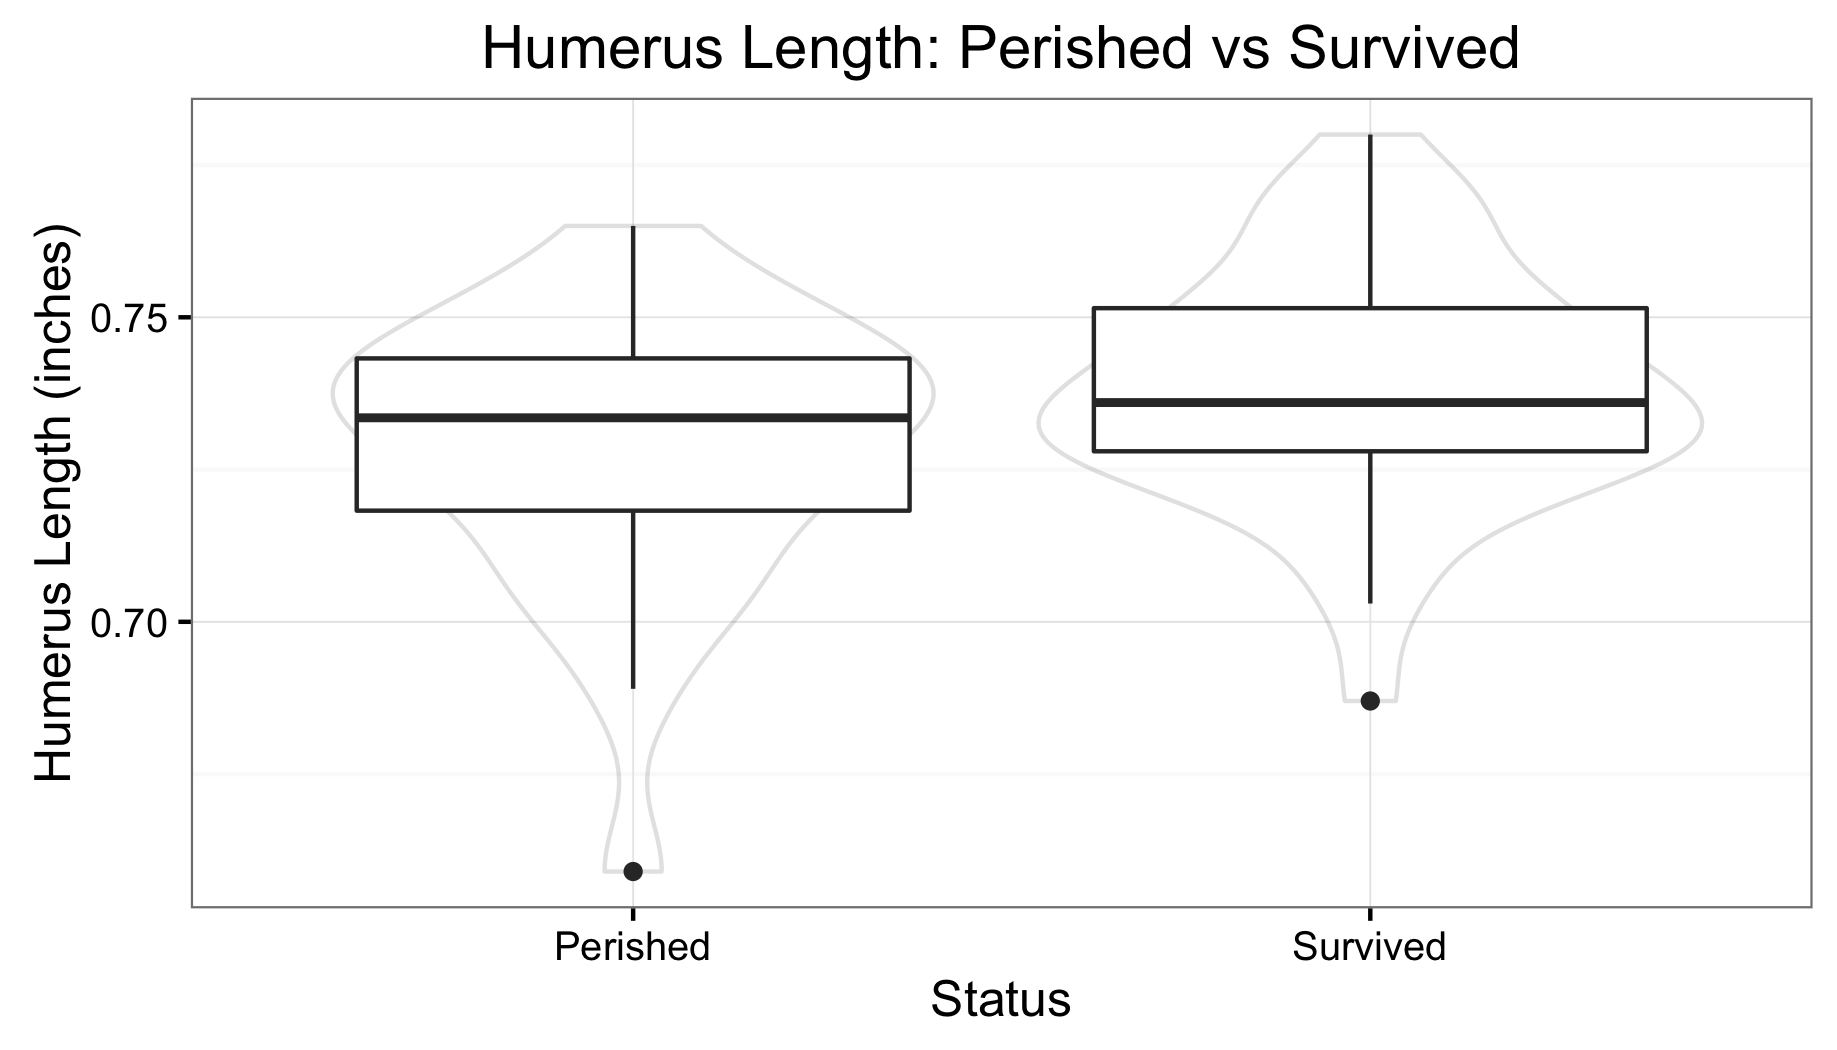
\includegraphics[width=4.25in]{4_full.png}
	\caption{Humerus lengths of male sparrows that perished or survived in a winter storm. The smallest length in the Perished group (indicated with a dot) is an extreme outlier and is later excluded from the analysis.}
	\label{fig:4}
\end{figure}


\titledquestion{\ramsey 3.32}

\textit{Analyze the data to describe the extent to which:}

\begin{parts}
\setlength{\parindent}{1em}

\part \textit{public school tuition is more expensive when out-of-state than when in-state.}

Boxplots of out-of-state vs in-state tuition for the 25 public schools (see Figure \ref{fig:5a_twoSample}) reveal (1) that out-of-state tuition has a higher center than in-state tuition, (2) that out-of-state tuition has a higher standard deviation than in-state tution, and (3) that some outliers may be skewing the results.
\begin{figure}
	\centering
	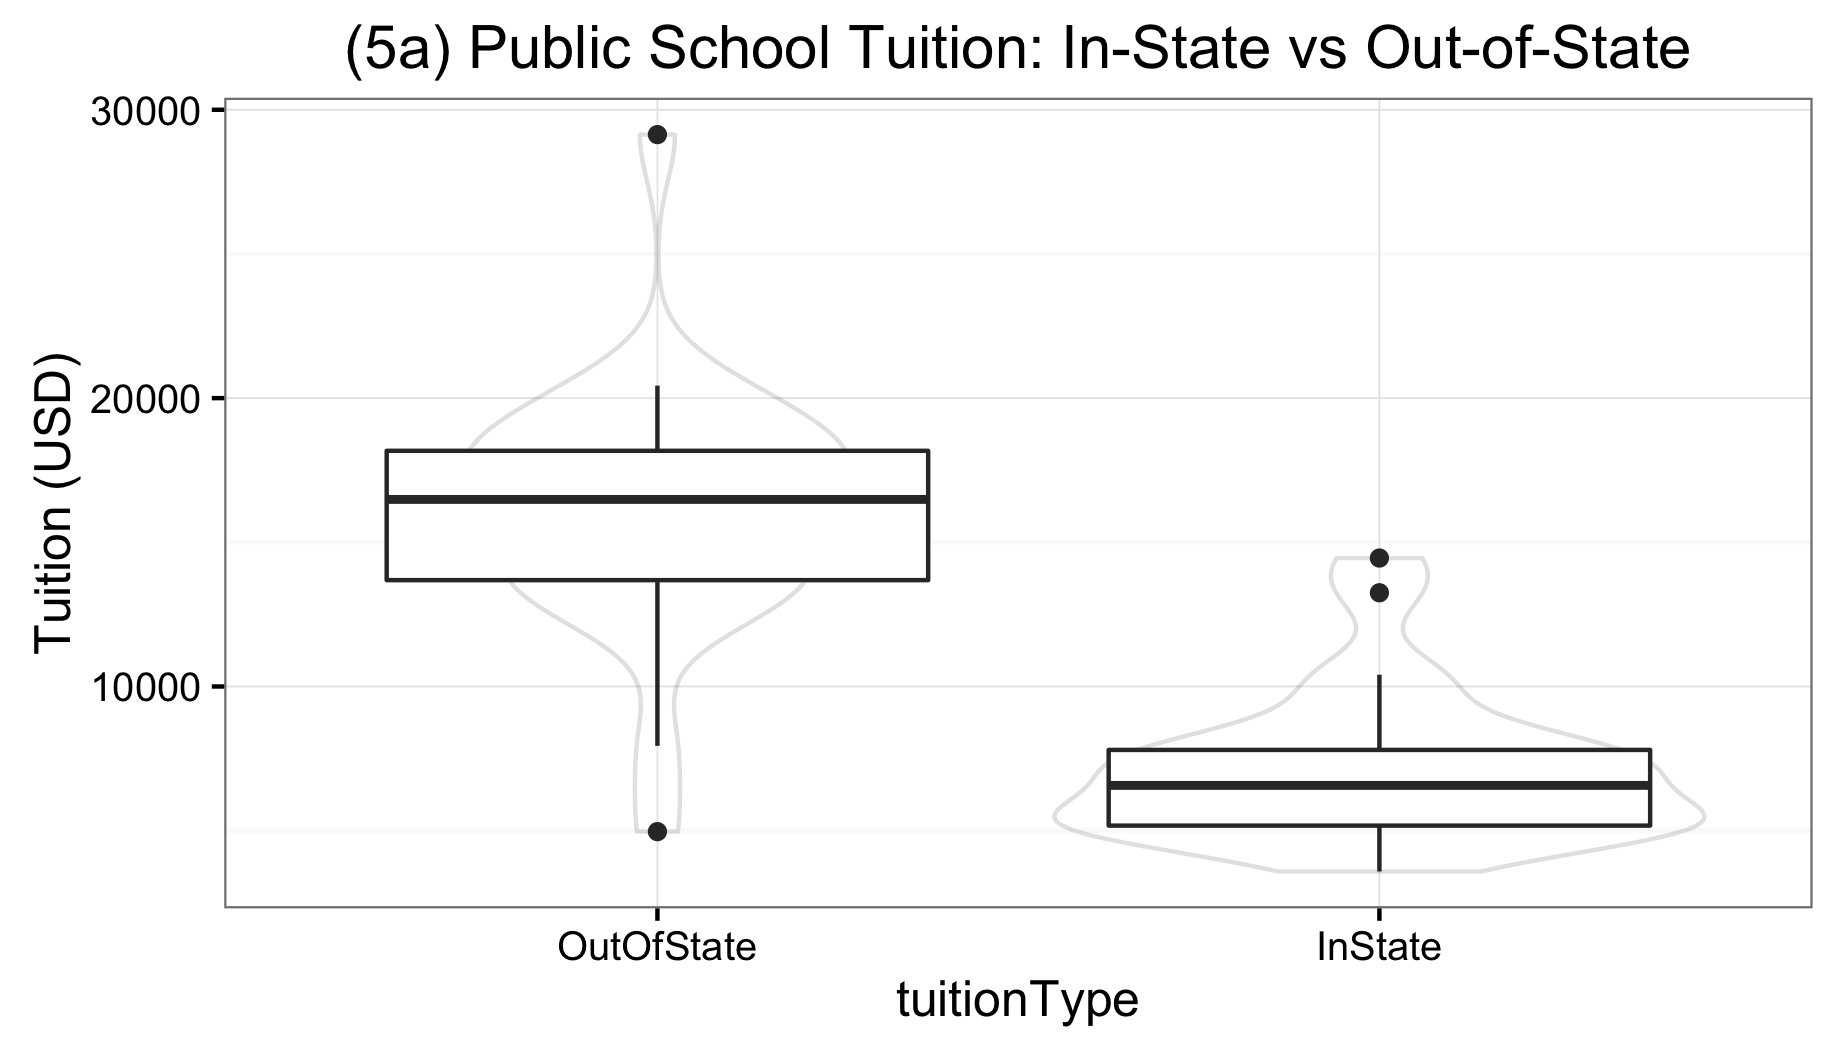
\includegraphics[width=4in]{5a_twoSample.png}
	\caption{Out-of-state vs in-state tuition costs for 25 public colleges.}
	\label{fig:5a_twoSample}
\end{figure}
The standard error for out-of-state tuition is 4,500.41 USD, which is 1.71 times higher than the standard error for in-state tuition of 2633.68 USD, making the two-sample t-tools unreliable here.

Luckily, the one-sample paired t-tools may be more appropriate in this case, since each \{out-of-state, in-state\} measurement is an observation on a single college. The distribution of the the difference between each \{out-of-state, in-state\} pair is nearly normal, as shown in Figure \ref{fig:5a_paired}.
\begin{figure}
	\centering
	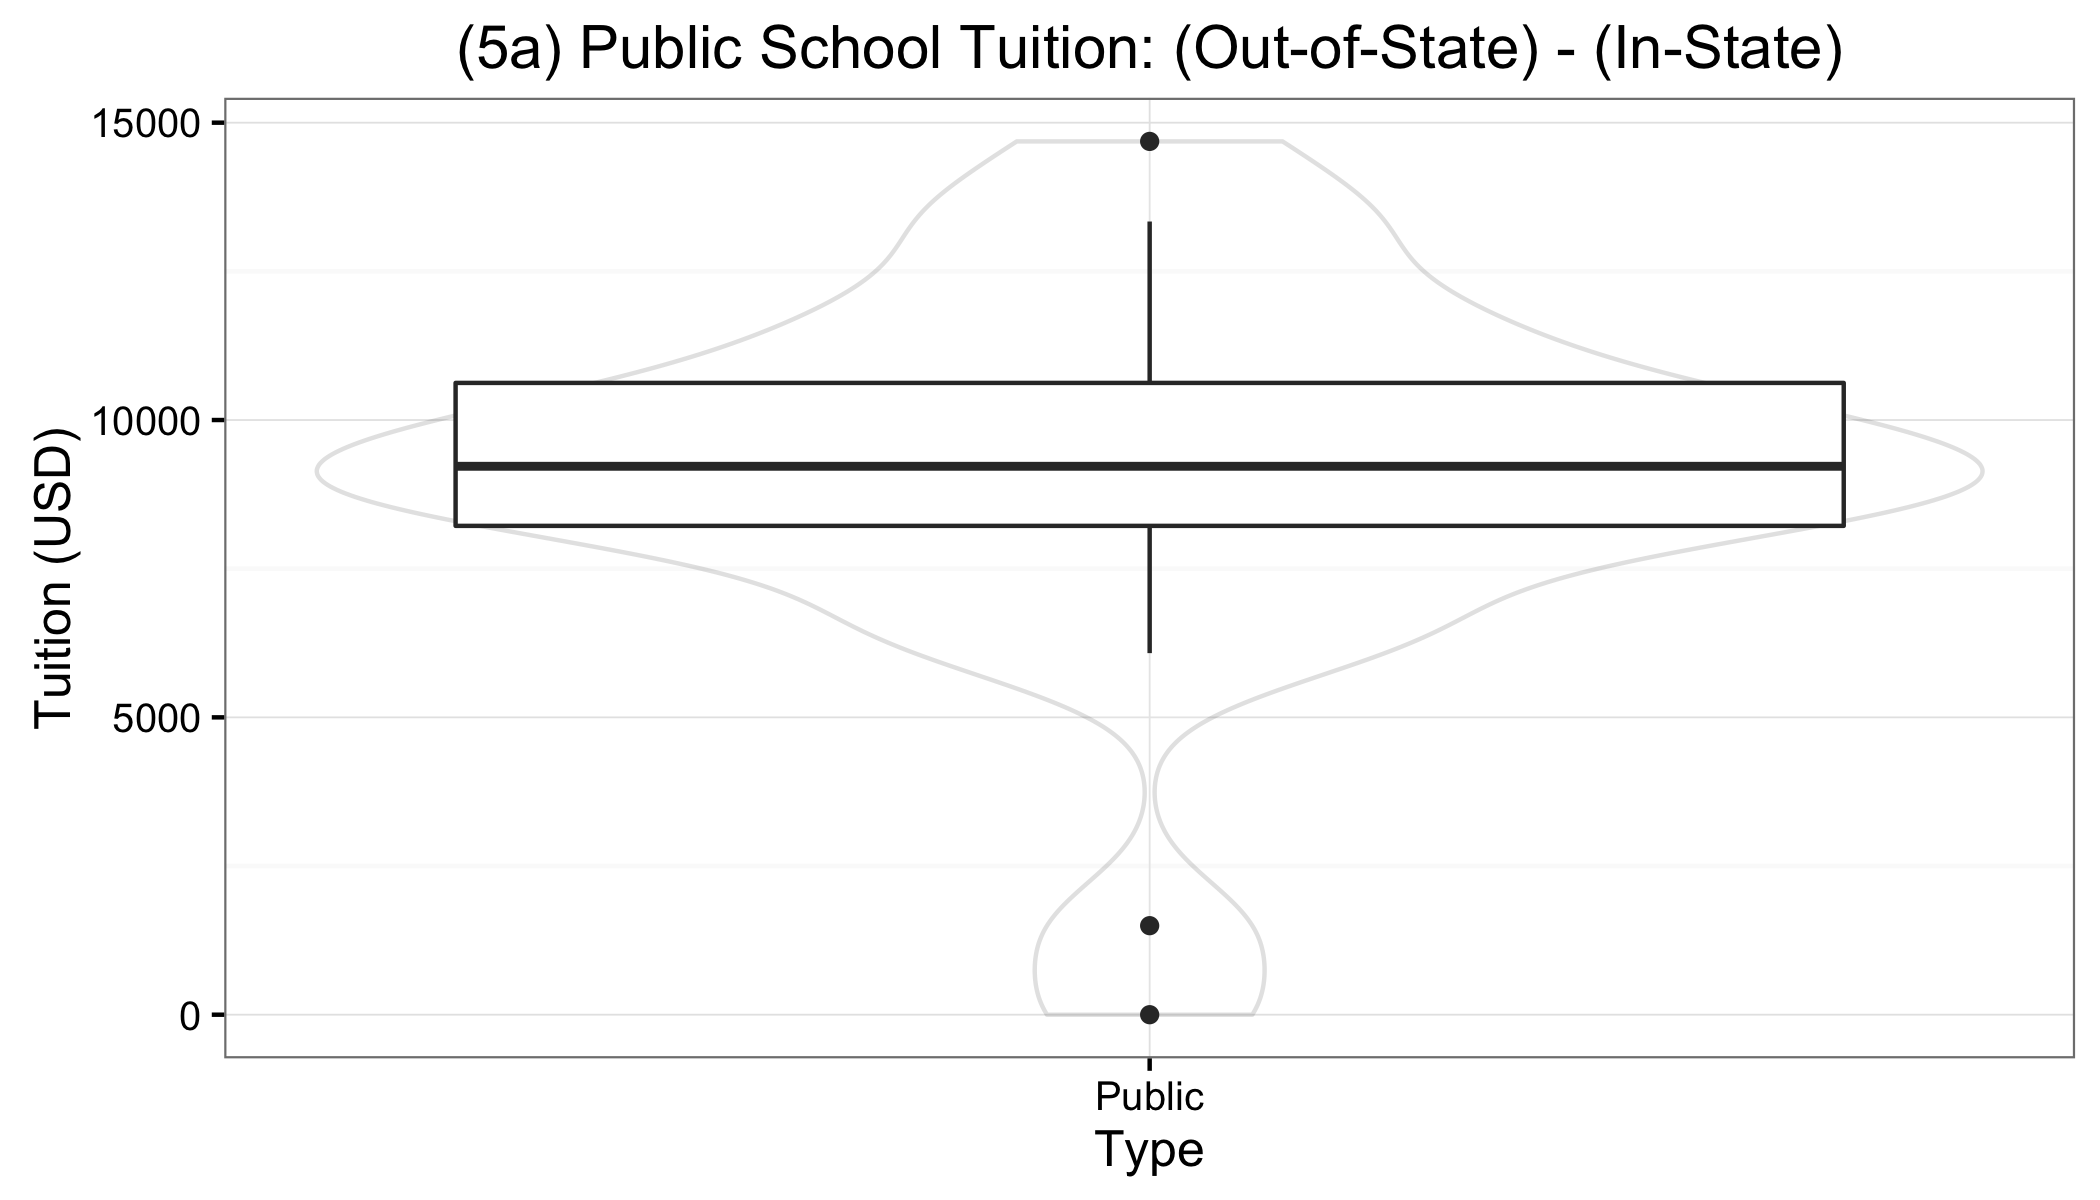
\includegraphics[width=4in]{5a_paired.png}
	\caption{(Out-of-state) - (in-state) tuition costs for 25 public colleges.}
	\label{fig:5a_paired}
\end{figure}
Using the paired t-test to test the alternative hypothesis that $\left(\text{out-of-state tuition}\right) - \left(\text{in-state tuition}\right) > 0$, we find substantial evidence that the mean difference in the out-of-state tuition and in-state tuition among a random sample of 25 public colleges is positive (one-sided p-value = $3.264\times10^{-13}$). It's estimated that the mean tuition cost is \$9,038.4 more for out-of-state tuition (95\% confidence interval: \$7,687.08 to \$10,389.72).



\part \textit{in-state tuition is more expensive for private schools than for public schools.}

Boxplots of in-state tuition costs for private vs public colleges (see Figure \ref{fig:5b_original}) reveal that private tuition has both a higher center and significantly higher spread than public tuition, making this dataset a good candidate for a log transformation.
\begin{figure}
	\centering
	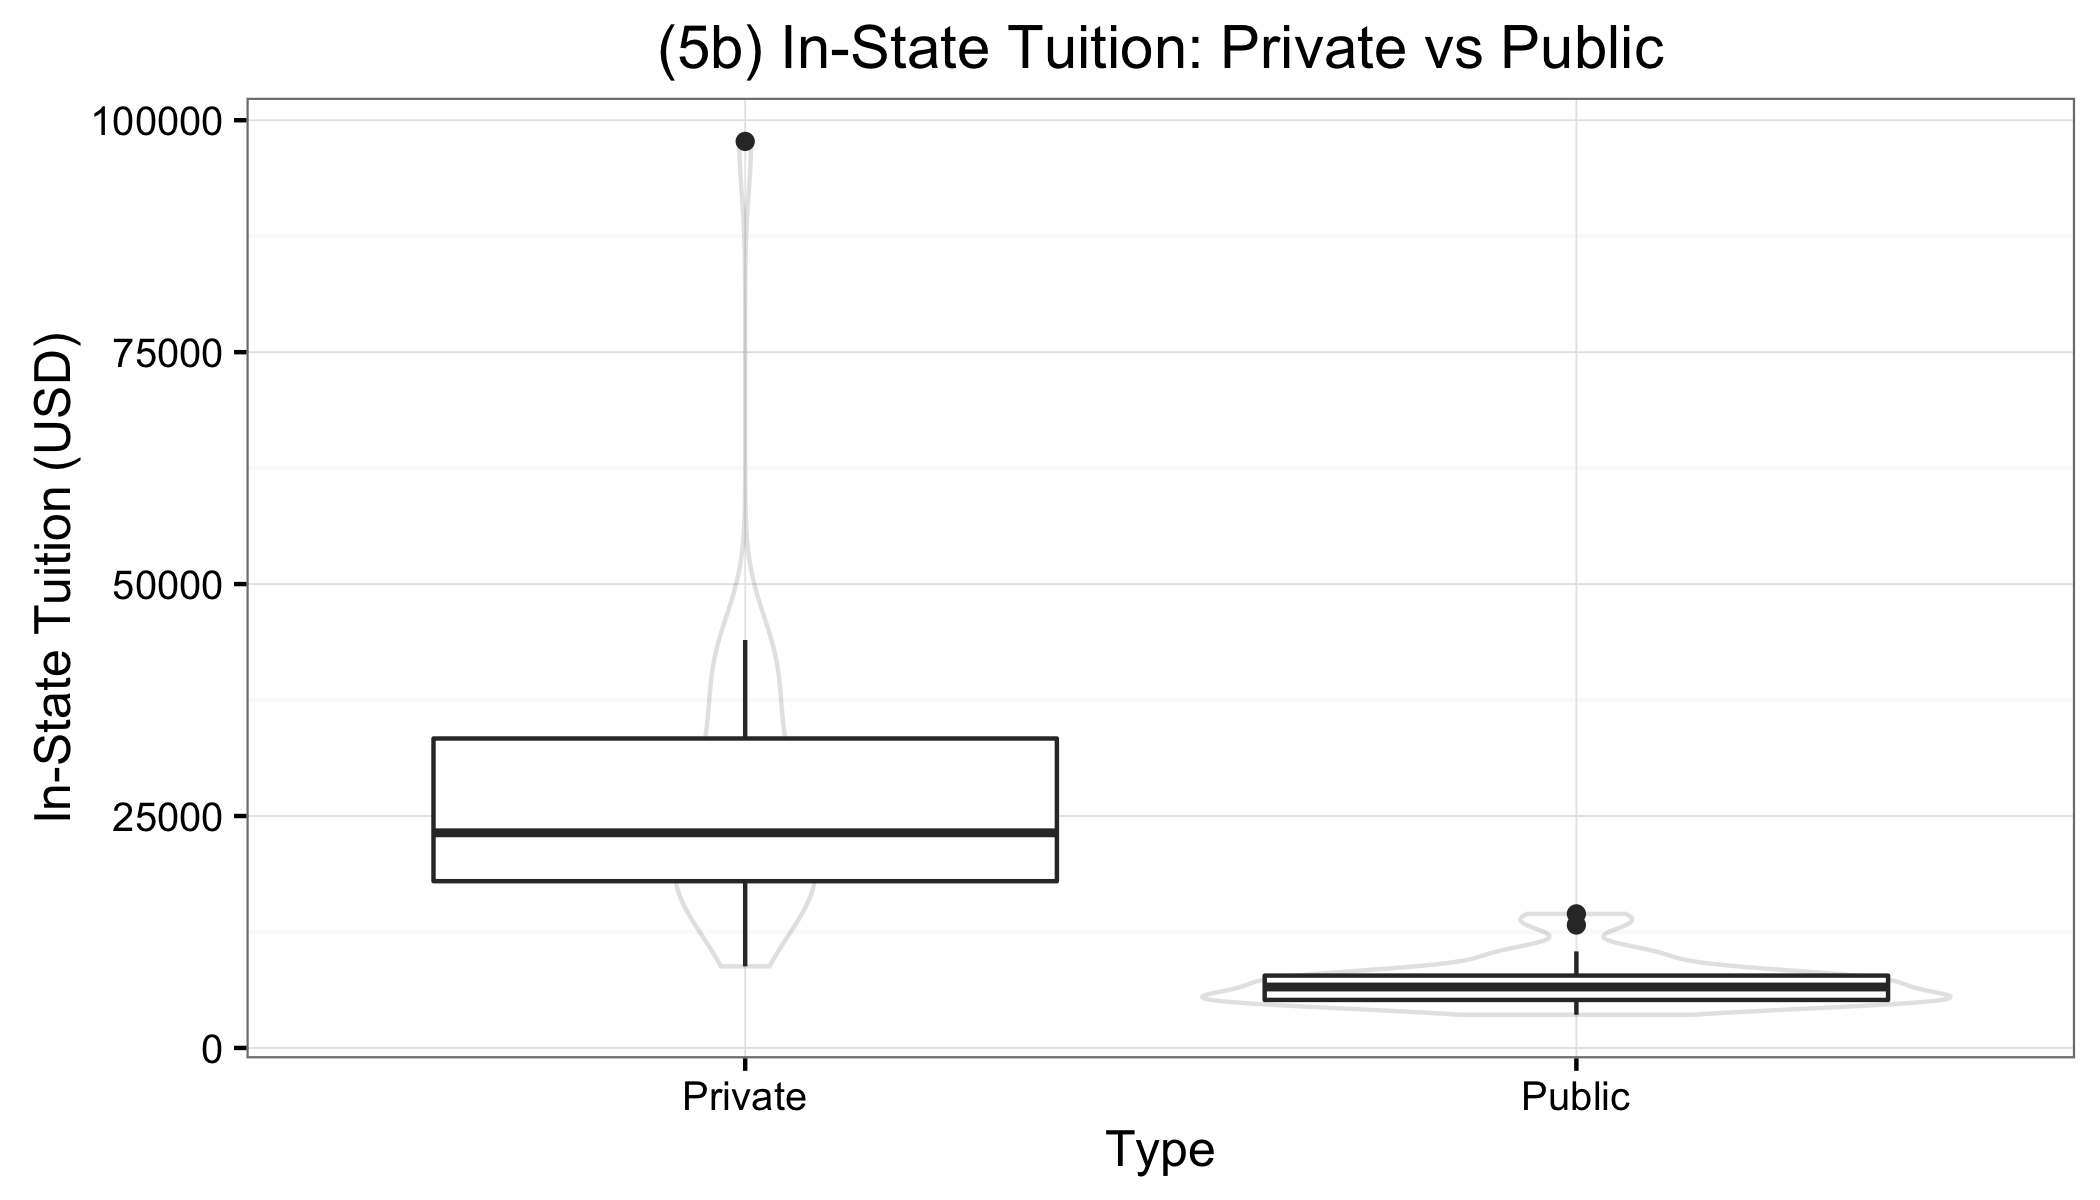
\includegraphics[width=4in]{5b_original.png}
	\caption{In-state tuition costs for private vs public colleges.}
	\label{fig:5b_original}
\end{figure}
The log-transformed data is shown in Figure \ref{fig:5b_log}, where the private tuition has a standard error of 0.495 and the public tuition has a similar standard error of 0.334 (on the log scale). Since the sample sizes in each group are the same, the the difference in standard errors has little effect on the robustness of the t-tools.
\begin{figure}
	\centering
	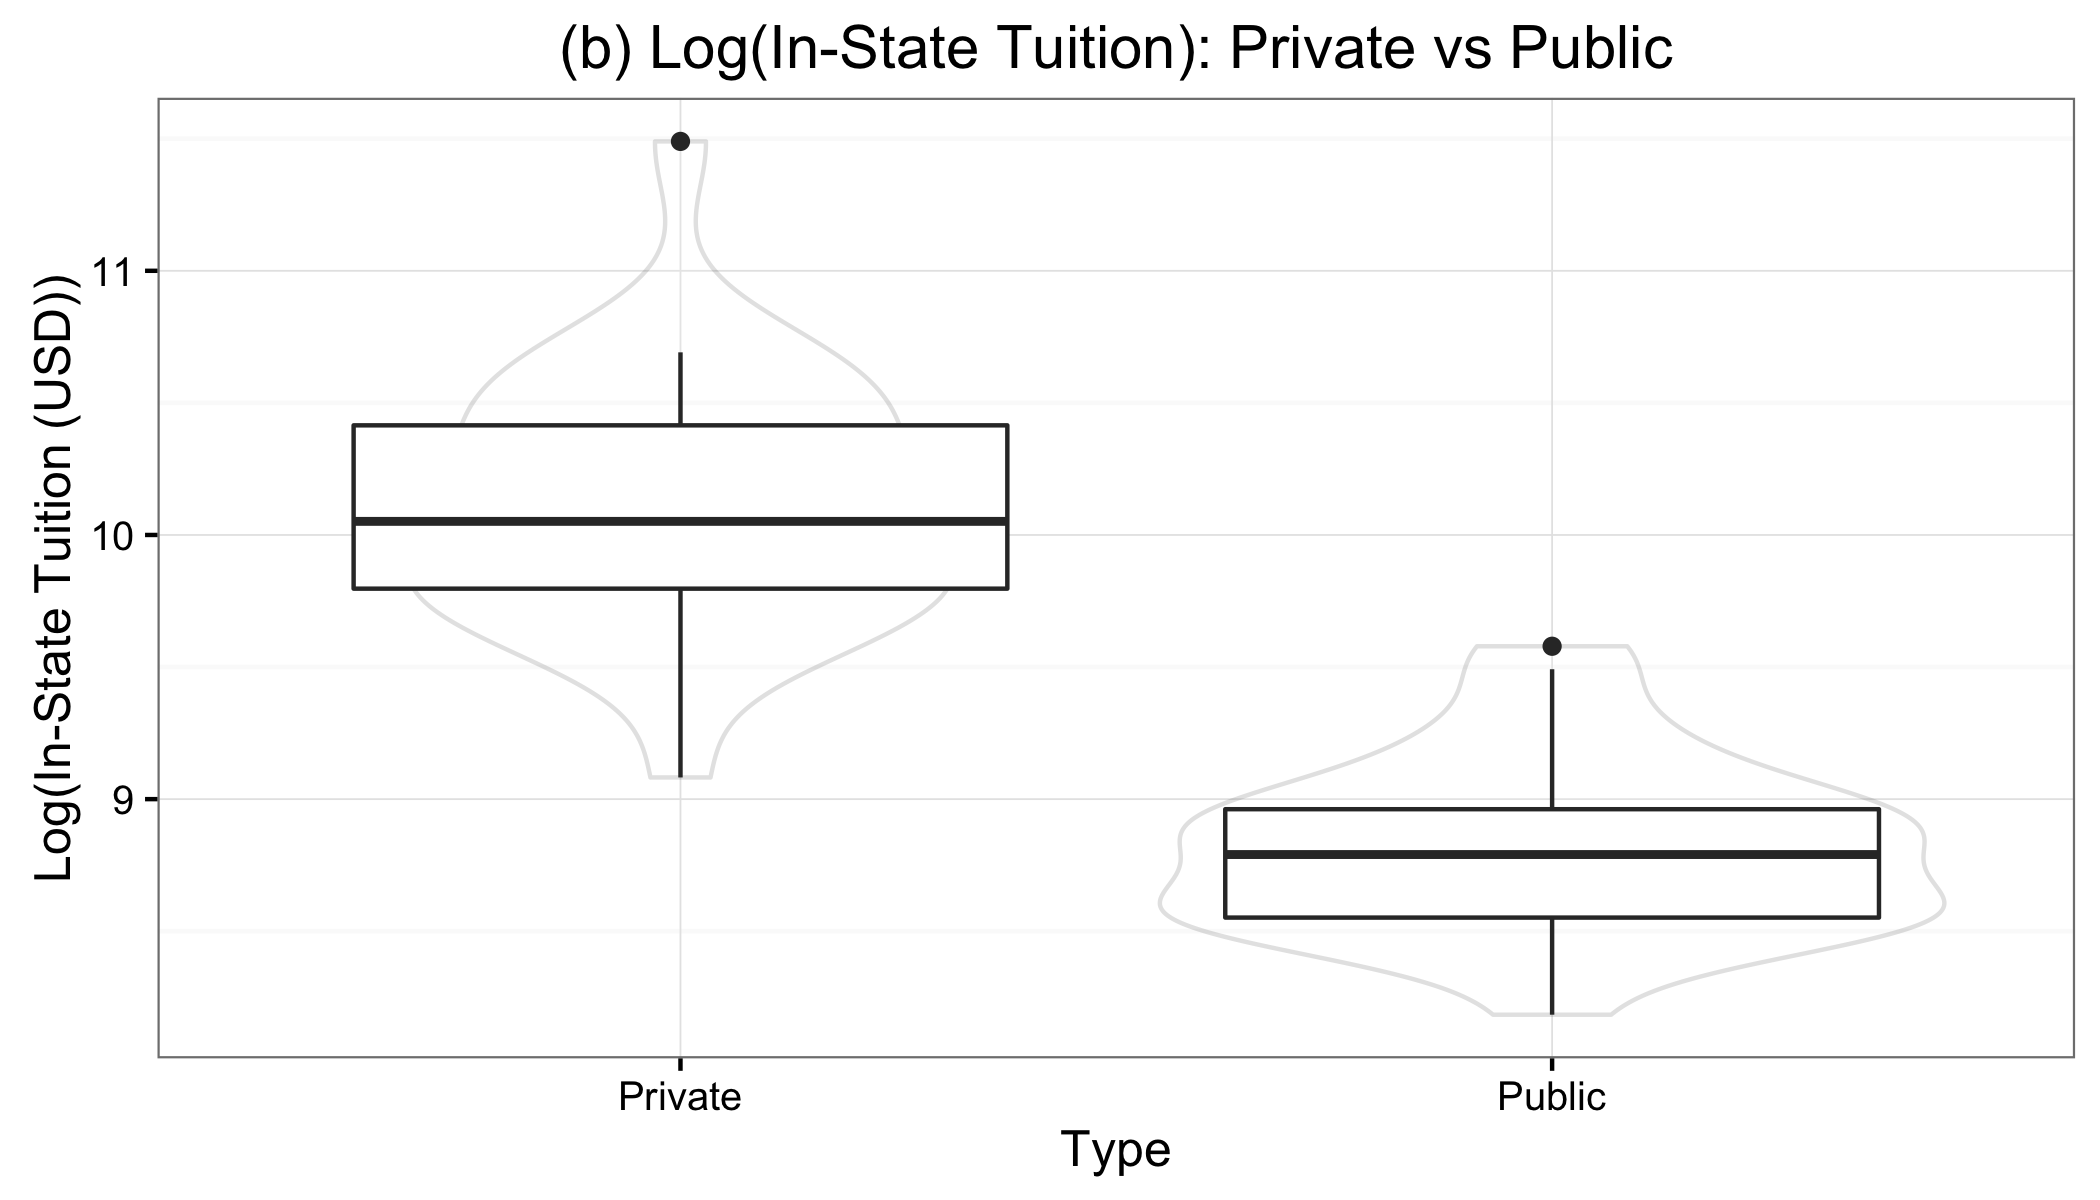
\includegraphics[width=4in]{5b_log.png}
	\caption{Log-transformed in-state tuition costs for private vs public colleges.}
	\label{fig:5b_log}
\end{figure}
Using the two-sample t-test on the log-transformed tuitions, we find substantial evidence that private school in-state tuition is greater than public school in-state tuition on the log scale (one-sided p-value: $6.31\times10^{-15}$). Back-transforming the estimate and confidence interval from the log scale to the original scale, it's estimated that the mean tuition cost is 3.692 times higher for out-of-state than in-state (95\% confidence interval: 2.904 to 4.695 times).




\part \textit{out-of-state tuition is more expensive for private schools than for public schools.}

Boxplots of out-of-state tuition costs for private vs public colleges (see Figure \ref{fig:5c_original}) reveal that private tuition has both a higher center and significantly higher spread than public tuition, making this dataset a good candidate for a log transformation.
\begin{figure}
	\centering
	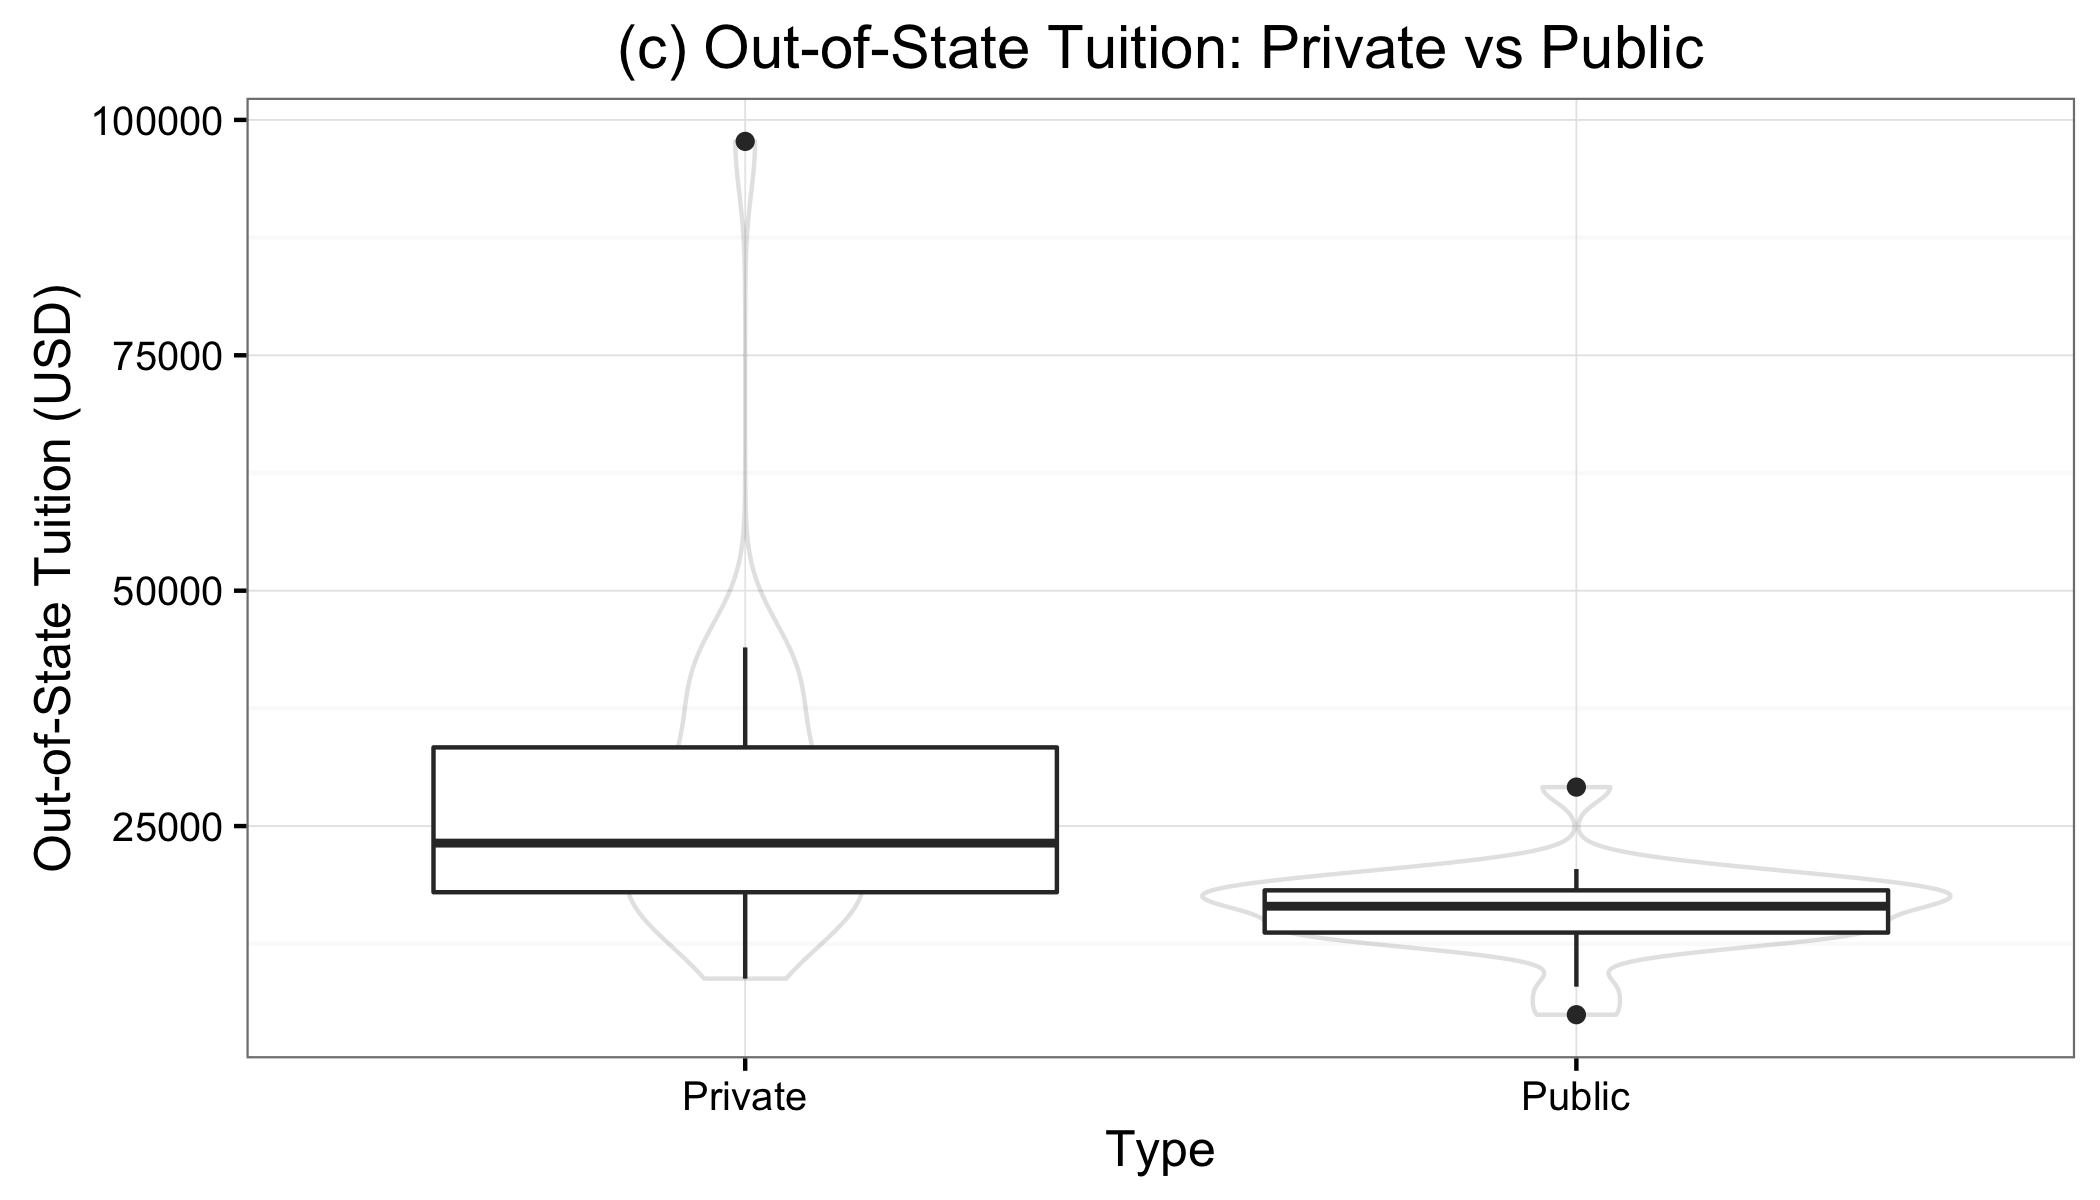
\includegraphics[width=4in]{5c_original.png}
	\caption{In-state tuition costs for private vs public colleges.}
	\label{fig:5c_original}
\end{figure}

The log-transformed data is shown in Figure \ref{fig:5c_log}, where the private tuition has a standard error of 0.495 and the public tuition has a similar standard error of 0.334 (on the log scale). Since the sample sizes in each group are the same, the the difference in standard errors has little effect on the robustness of the t-tools.
\begin{figure}
	\centering
	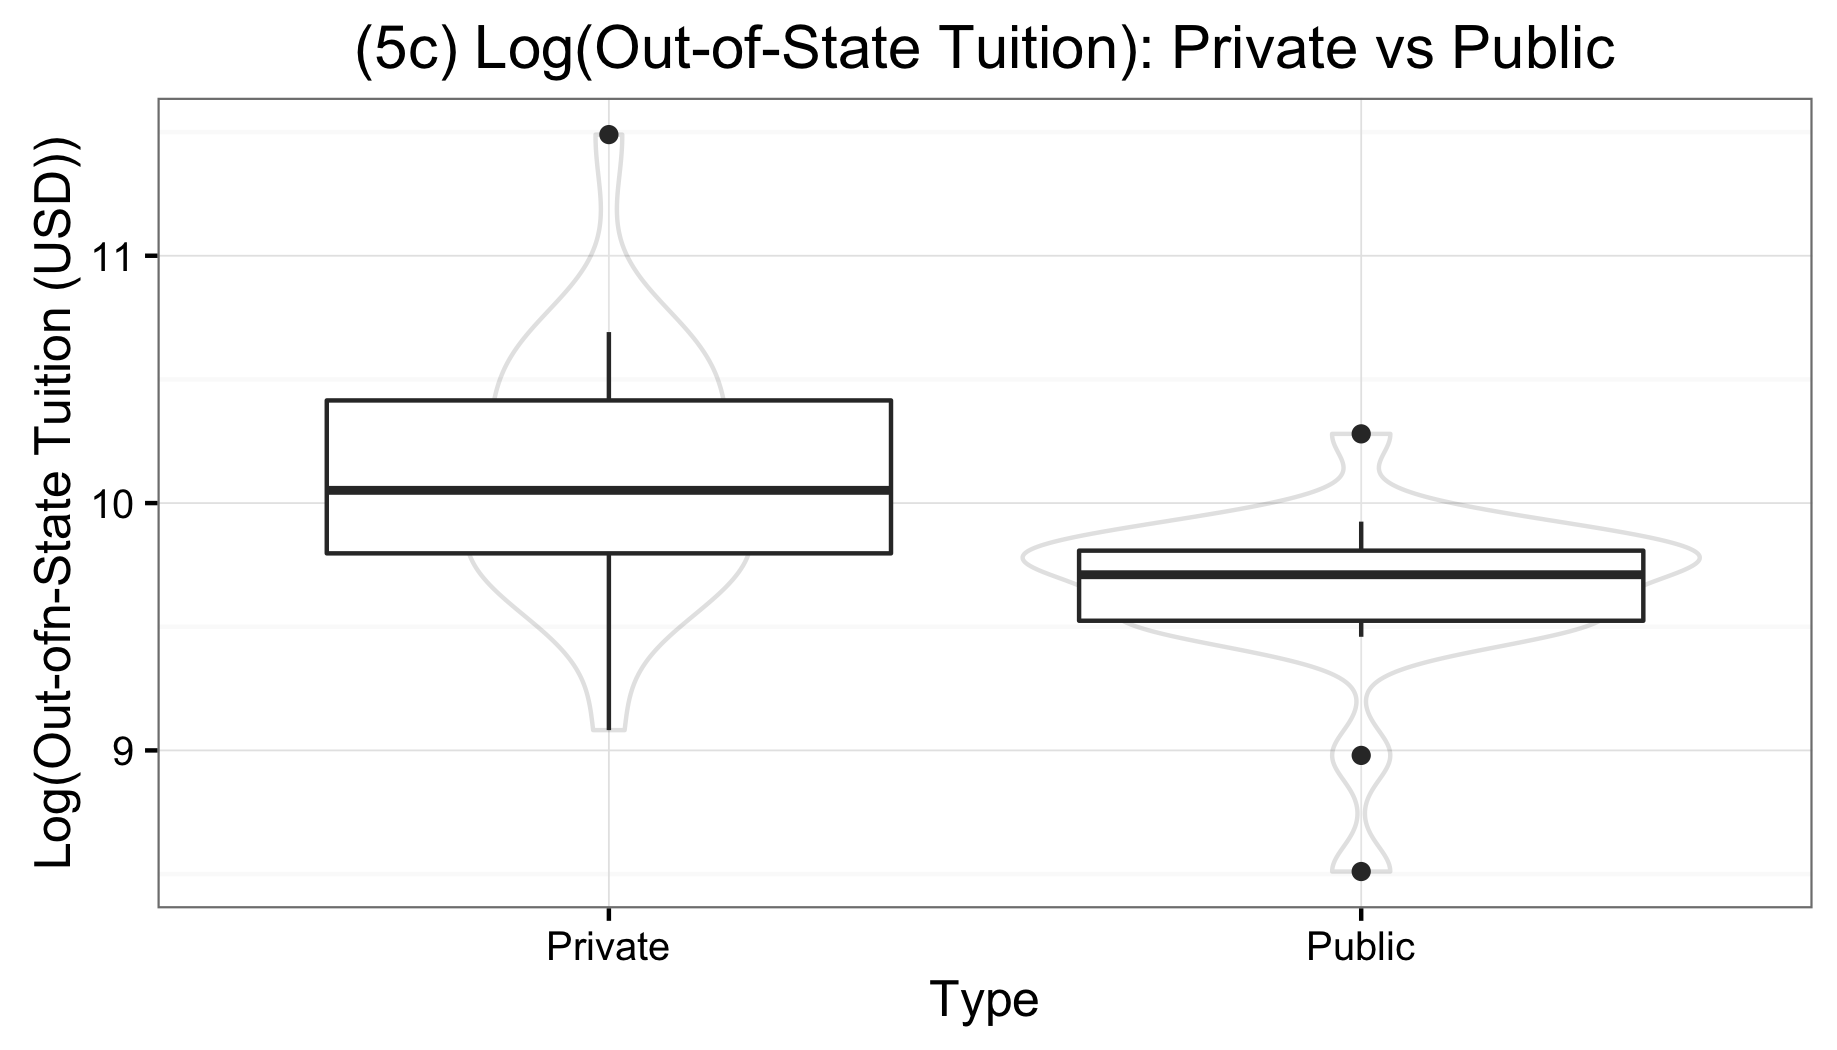
\includegraphics[width=4in]{5c_log.png}
	\caption{Log-transformed out-of-state tuition costs for private vs public colleges.}
	\label{fig:5c_log}
\end{figure}
Using the two-sample t-test on the log-transformed tuitions, we find substantial evidence that private school in-state tuition is greater than public school in-state tuition on the log scale (one-sided p-value: $0.0001073$). Back-transforming the estimate and confidence interval from the log scale to the original scale, it's estimated that the mean tuition cost is  1.613 times higher for out-of-state than in-state (95\% confidence interval: 1.269 2.0512 times).


\end{parts}


\titledquestion{\ramsey 4.19}

Using the \texttt{wilcox.test} R function:

\begin{codeSmall}
> # load data
> sparrowData <- Sleuth3::ex0221
> 
> # perform rank-sum test
> wilcox.test(formula=Humerus~Status, data=sparrowData,
+             paired=FALSE, # perform rank-sum test
+             correct=TRUE, # apply continuity correction in the normal approx for the p-value
+             conf.int=TRUE, conf.level=0.95)

	Wilcoxon rank sum test with continuity correction

data:  Humerus by Status
W = 331, p-value = 0.1718
alternative hypothesis: true location shift is not equal to 0
95 percent confidence interval:
 -0.019076357  0.003033795
sample estimates:
difference in location 
          -0.007022596 

Warning messages:
1: In wilcox.test.default(x = c(0.659, 0.689, 0.703, 0.702, 0.709,  :
  cannot compute exact p-value with ties
2: In wilcox.test.default(x = c(0.659, 0.689, 0.703, 0.702, 0.709,  :
  cannot compute exact confidence intervals with ties
\end{codeSmall}


\begin{parts}
\setlength{\parindent}{1em}


\part The two-sided p-value is 0.1718.

\part From the documentation, by default, when the \texttt{exact} argument isn't specified the \texttt{wilcox.test} function computes an exact p-value only when the combined sample has fewer than 50 values and there are no ties. Otherwise, as is the case here, since our dataset has 59 observations and also has ties, a normal approximation is used.

\part The p-value based on the normal approximation uses a continuity correction to the Z-statistic.

\part The (two-sided) p-value from the rank-sum test (0.1718) is greater than the p-value from the two-sample t-test (0.0809) and slightly smaller than the p-value from the two-sample t-test when the smallest observation is excluded (0.18) in Problem \ref{ques:ramsey0328}.

\part In this case, the (two-sided) p-value obtained from the two-sample t-test when excluding outliers is nearly identical to the p-value obtained in the rank-sum test.

The two-sample t-test assumes nearly normal populations, equal population variances, and independence of samples. All of these assumptions are nearly satisfied both when the outlier is and isn't excluded.

By design, the rank-sum test less efficient when the populations are normal, but is much better at dealing with outliers and makes no assumption about the population distributions. 

Removing the outlier isn't entirely justified here --- there isn't any indication that there were recording errors or that the outlier came from a different population --- so the rank-sum test may be a better choice, since it generates a similar p-value and entirely avoids the issue of excluding outliers.

\end{parts}


\end{questions}

%\listoftodos

\end{document}